\documentclass[12pt,titlepage]{article}
\usepackage[margin=1.25in]{geometry}
\usepackage{graphicx,amsmath,blindtext,minted}

%% Variables definition
\newcommand{\vSubject}{Web Design and Development}
\newcommand{\vSubtitle}{Javascript}
\newcommand{\vName}{Muhammad Baihaqi Aulia Asy'ari}
\newcommand{\vNIM}{2241720145}
\newcommand{\vClass}{2I}
\newcommand{\vDepartment}{Information Technology}
\newcommand{\vStudyProgram}{D4 Informatics Engineering}

%% [START] Tikz related stuff
\usepackage{tikz}
\usetikzlibrary{svg.path,calc,shapes.geometric,shapes.misc}
\tikzstyle{terminator} = [rectangle, draw, text centered, rounded corners = 1em, minimum height=2em]
\tikzstyle{preparation} = [chamfered rectangle, chamfered rectangle sep=0.75em, draw, text centered, minimum height = 2em]
\tikzstyle{process} = [rectangle, draw, text centered, minimum height=2em]
\tikzstyle{decision} = [diamond, aspect=2, draw, text centered, minimum height=2em]
\tikzstyle{data}=[trapezium, draw, text centered, trapezium left angle=60, trapezium right angle=120, minimum height=2em]
\tikzstyle{connector} = [line width=0.25mm,->]
%% [END] Tikz related stuff

%% [START] Fancy header related stuff
\usepackage{fancyhdr}
\pagestyle{fancy}
\setlength{\headheight}{15pt} % compensate fancyhdr style
\fancyhead{}
\fancyfoot{}
\fancyfoot[L]{\thepage}
\fancyfoot[R]{\textit{\vSubject - \vSubtitle}}
\renewcommand{\footrulewidth}{0.4pt}% default is 0pt, overline for footer
%% [END] Fancy header related stuff

%% [START] Custom tabular command related stuff
\usepackage{tabularx}
\newcommand{\details}[2]{
    #1 & #2  \\
}
%% [END] Custom tabular command related stuff

%% [START] Figure related stuff
\newcommand{\image}[3][1]{
    \begin{figure}[h]
        \centering
        \includegraphics[#1]{#2}
        \caption{#3}
        \label{#3}
    \end{figure}
}
%% [END] Figure related stuff

%%
\usepackage{pgf-umlcd}

\renewcommand{\umldrawcolor}{black}
\renewcommand{\umlfillcolor}{white}
%%

%% [BEGIN] Custom enumerator
\usepackage{enumitem}
%% [END] Custom enumerator

%% [BEGIN] Paragraph indent
\usepackage{indentfirst}
%% [END] Paragraph indent

\begin{document}
\begin{titlepage}
    \centering
    \vfill
    {\bfseries\LARGE
        \vSubject\\
        \vskip0.25cm
        \vSubtitle
    }
    \vfill
    
\includegraphics[width=6cm]{images/polinema-logo.png}
    \vfill
    {
        \textbf{Name}\\
        \vName\\
        \vskip0.5cm
        \textbf{NIM}\\
        \vNIM\\
        \vskip0.5cm
        \textbf{Class}\\
        \vClass\\
        \vskip0.5cm
        \textbf{Department}\\
        \vDepartment\\
        \vskip0.5cm
        \textbf{Study Program}\\
        \vStudyProgram
    }
\end{titlepage}

\newpage

\begin{enumerate}
    \subsection*{Practicum 1 - Intro}
    \item - \\ \includegraphics[width=.9\textwidth]{images/figures/fig1.png} \\ there is an alert from the browser after typing in the command alert in the console
    \subsection*{Practicum 2 - First Javascript Program}
    \item There is hello world written on the HTML page.
    \item The console log appears in the console tab. \\ \includegraphics[width=.9\textwidth]{images/figures/fig2.png}
    \item Because console log print text in the console. 
\end{enumerate}

\subsection*{Practicum 3 - Writing Javascript Code in HTML}

\subsubsection*{1. Embed Javascript}
\begin{enumerate}
    \item - \\ 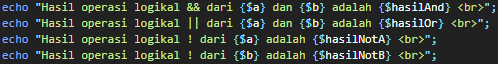
\includegraphics[width=.9\textwidth]{images/figures/fig3.png} \\ both script in head and body executed in top down order. 
    \item i think the body is better because then the whole html (atleast the part that are about to be manipulated by the javascript) finish load. in result the javascript executed faster because it doesnt need to wait for the html element it about to use to load first. 
\end{enumerate}

\subsubsection*{2. Inline Javascript}
\begin{enumerate}
    \item - \\ \includegraphics[width=.9\textwidth]{images/figures/fig4.png} \\ both anchor creat an alert in the browser. 
    \item one use the href to run the javascript, the other use onclick attribute. 
\end{enumerate}

\subsubsection*{3. External Javascript}
\begin{enumerate}
    \item - \\ 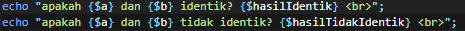
\includegraphics[width=.9\textwidth]{images/figures/fig5.png} \\ the alert load in first, but after inspecting the page, the html is partially loaded up to the script tag.
    \item the script did not load like before.
    \subsection*{Practicum 4 - Dialog Window}
    \item - \\ 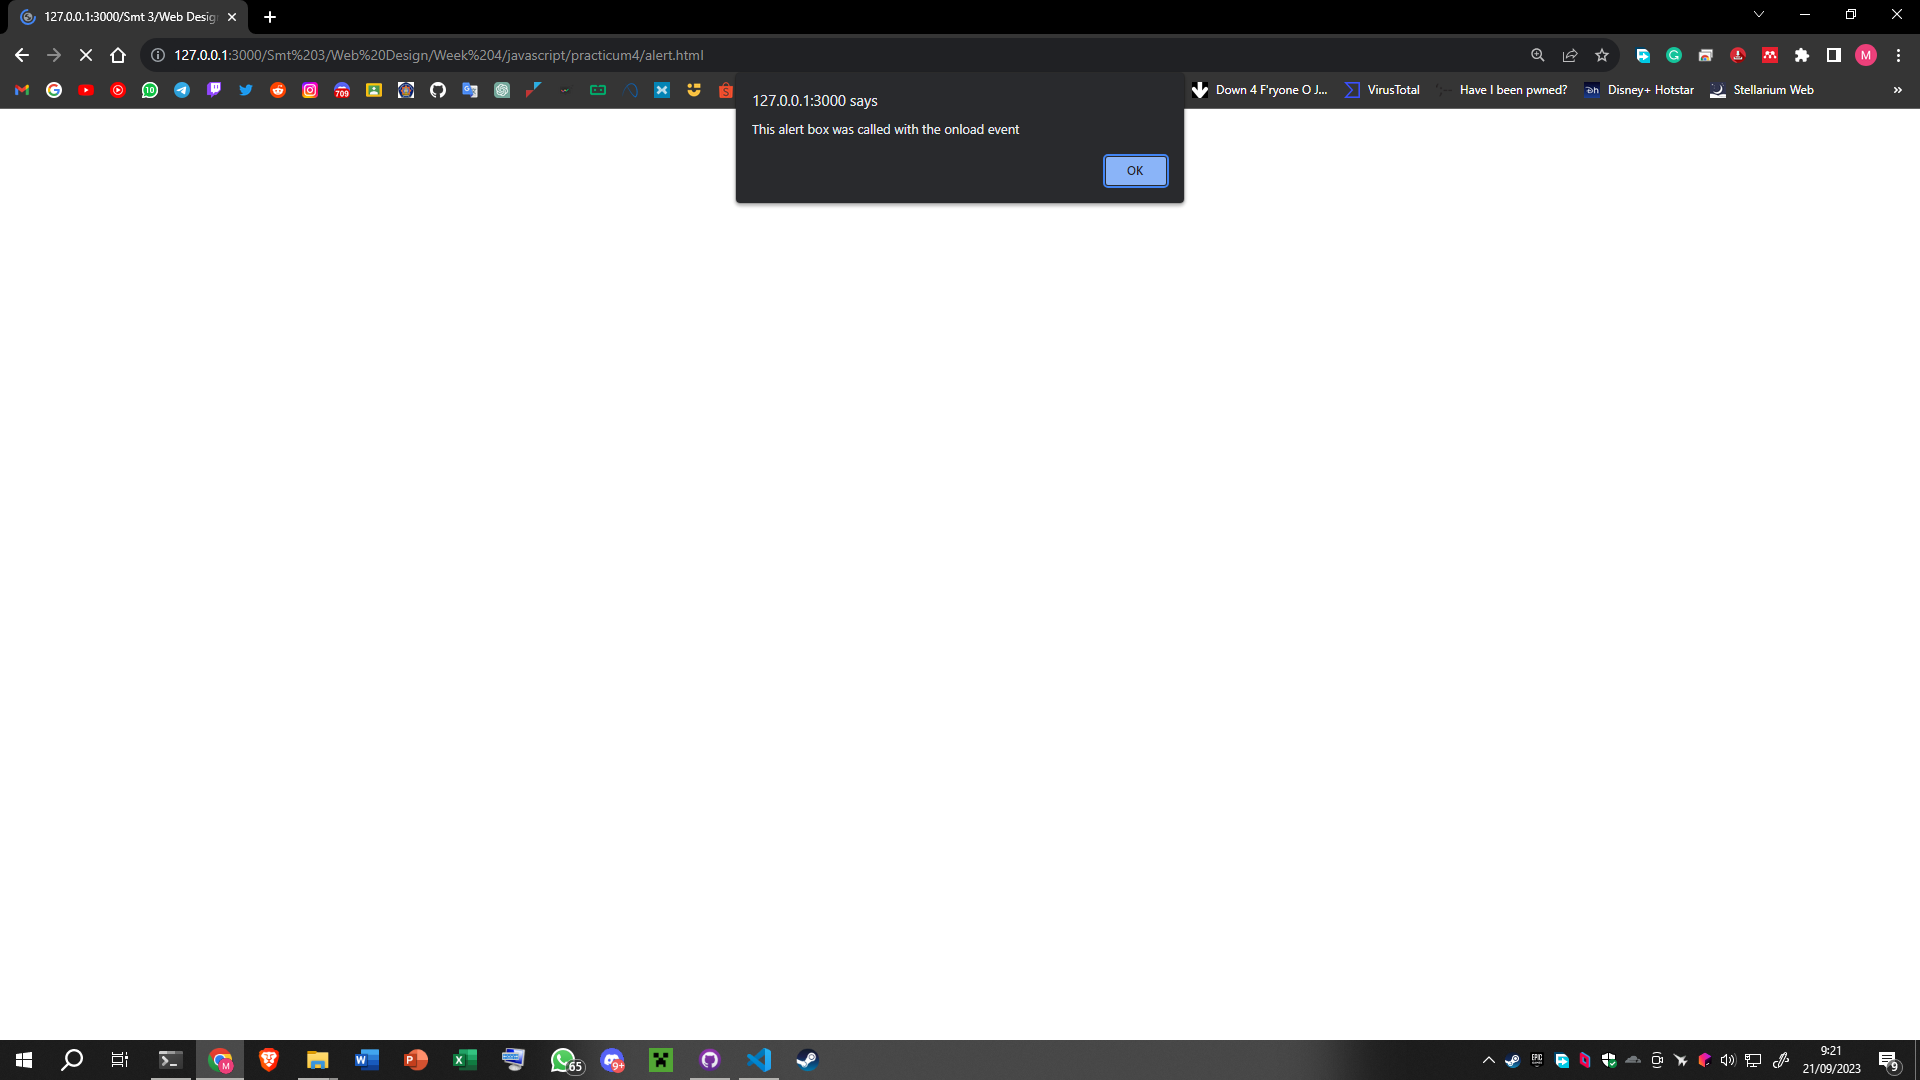
\includegraphics[width=.9\textwidth]{images/figures/fig6.png} \\ an alert show up uppon the page load.
    \item - \\ \includegraphics[width=.9\textwidth]{images/figures/fig7.png} \\ the browser gave me an option to go to the polinema website or cancel it in which when canceling the script tag write text on the page.
    \newpage
    \item - \\ \includegraphics[width=.9\textwidth]{images/figures/fig8.png} \\ 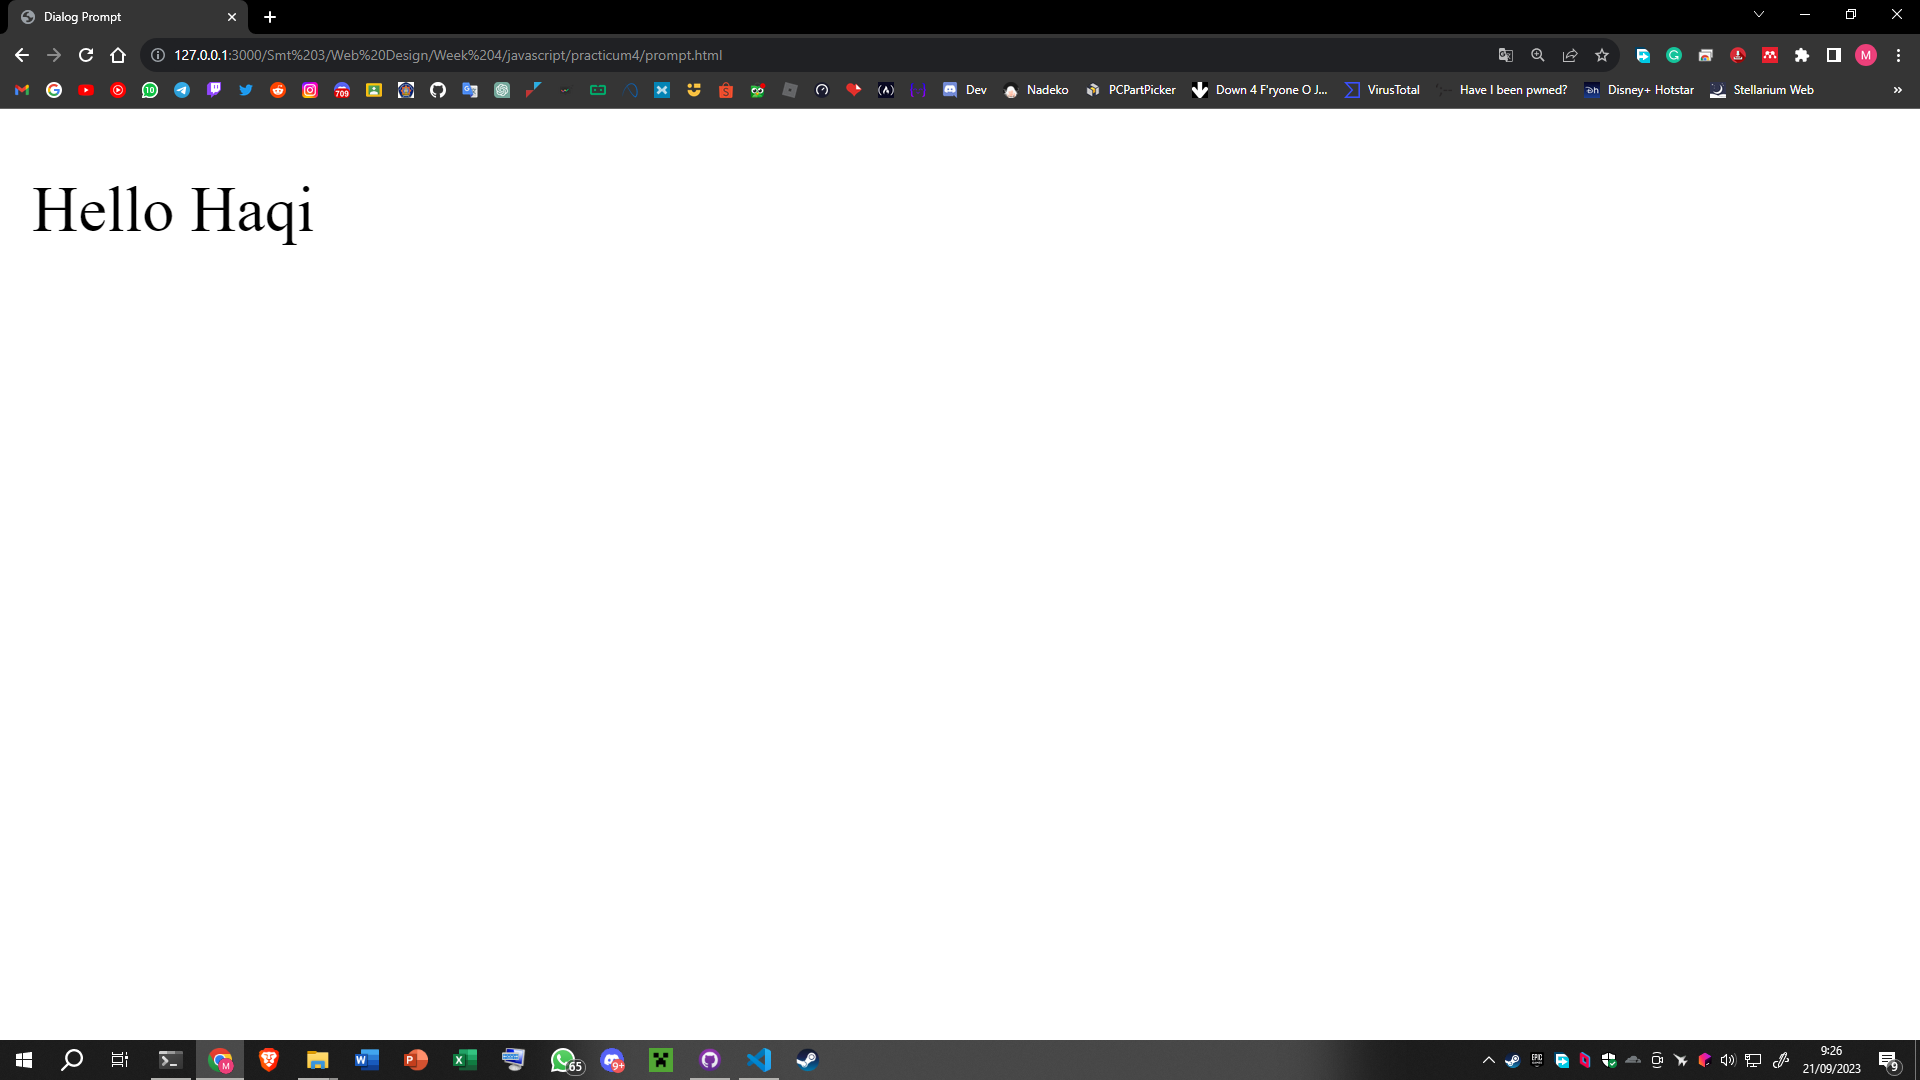
\includegraphics[width=.9\textwidth]{images/figures/fig9.png} \\ the browser prompted me with the parameter that have been set in the prompt function inside the script tag.
    \subsection*{Practicum 5 - Variables}
    \item - \\ 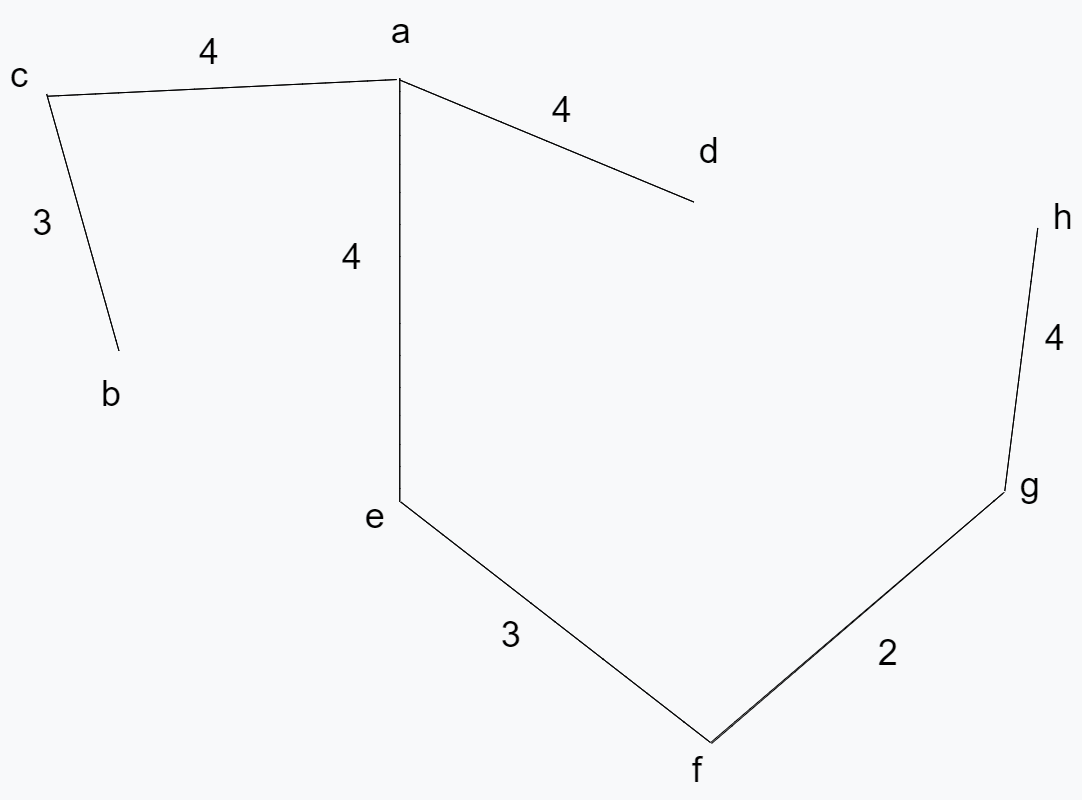
\includegraphics[width=.9\textwidth]{images/figures/fig10.png} \\ the var can be written inside the html document.
    \subsection*{Practicum 6 - Functions}
    \item - \\ 
\includegraphics[width=.9\textwidth]{images/figures/fig11.png} \\ uppon clicking the anchor, the browser alerted me with hello world.
    \newpage
    \item - \\ 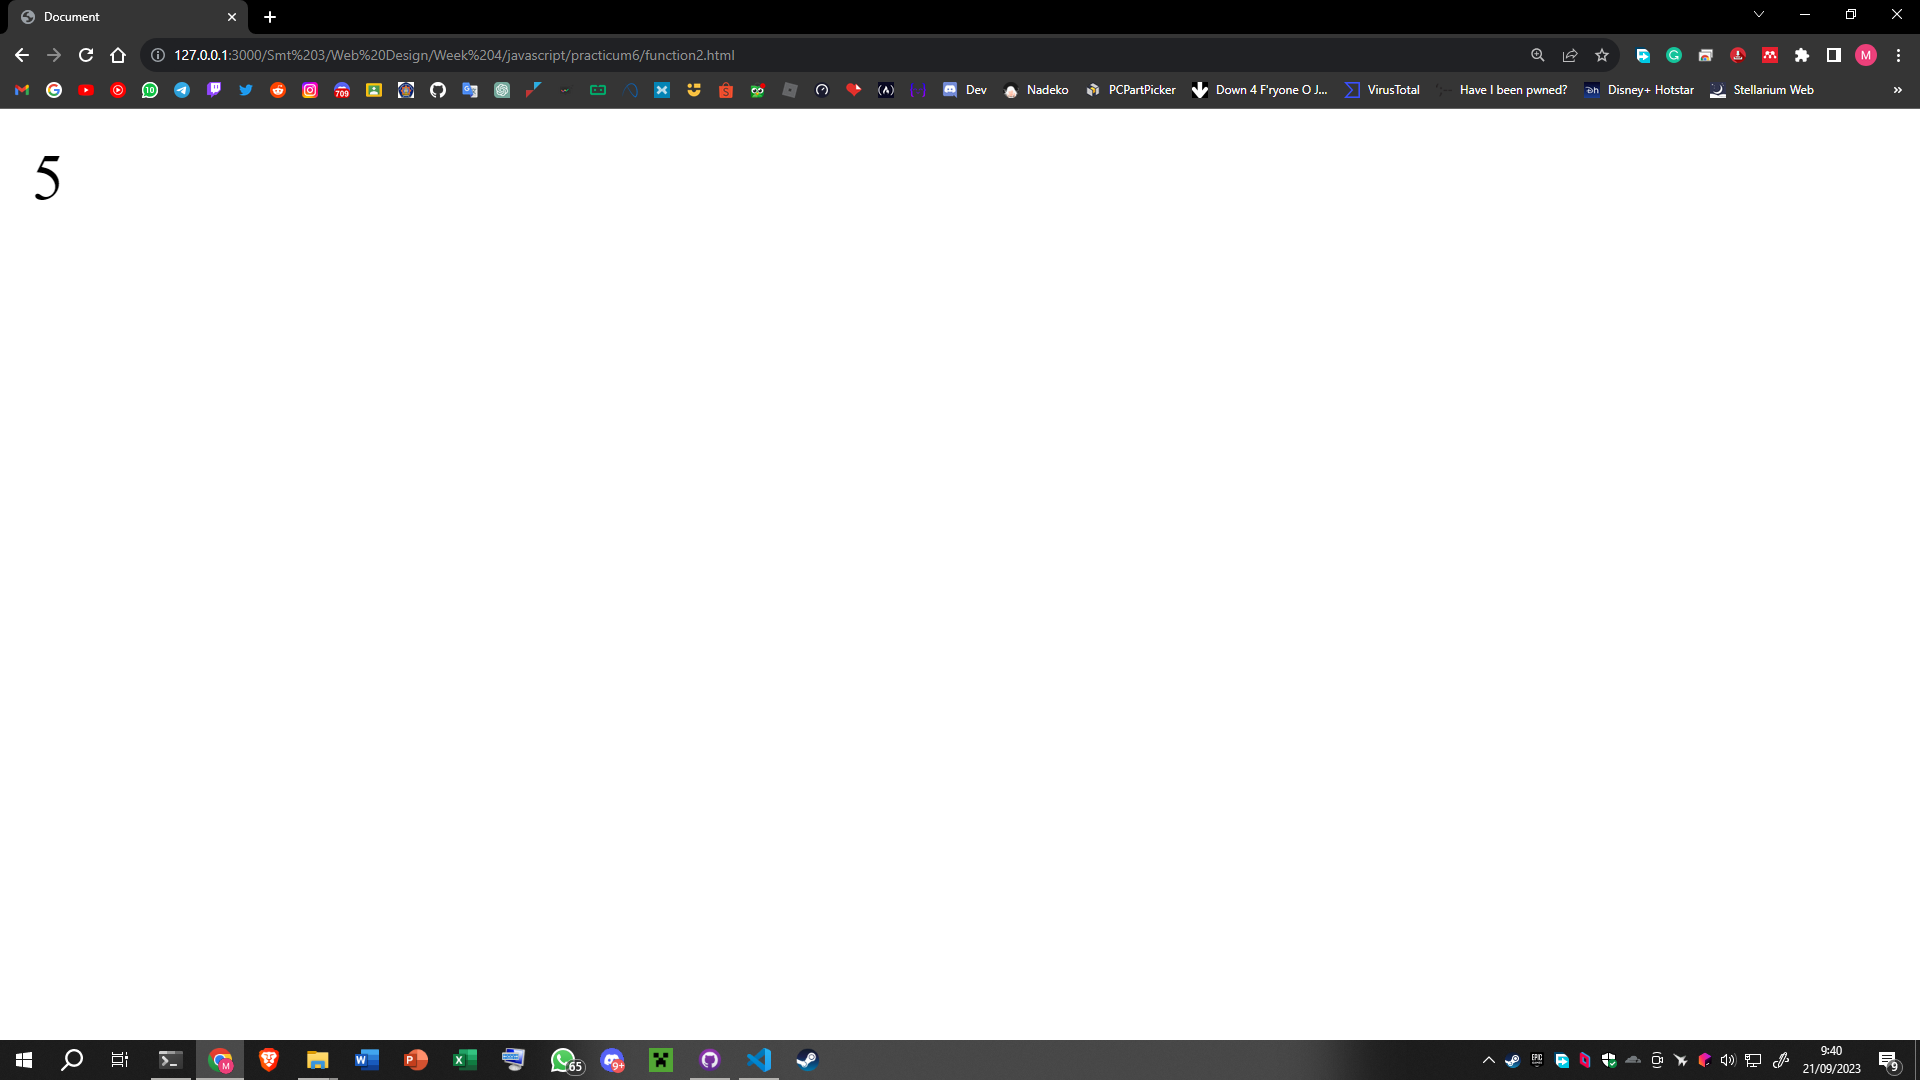
\includegraphics[width=.9\textwidth]{images/figures/fig12.png} \\ the browser write the result of the function after it being called in the script tag in the page body.
    \subsection*{Practicum 7 - Data Types}
    \item - \\ \includegraphics[width=.9\textwidth]{images/figures/fig13.png} \\ javascript is dynamically typed, one can declare a variable and be replaced with different data type with out casting the data.
    \newpage
    \item - \\ \includegraphics[width=.9\textwidth]{images/figures/fig14.png} \\ there are many ways to declare a string with quote mark inside of a string
    \item - \\ 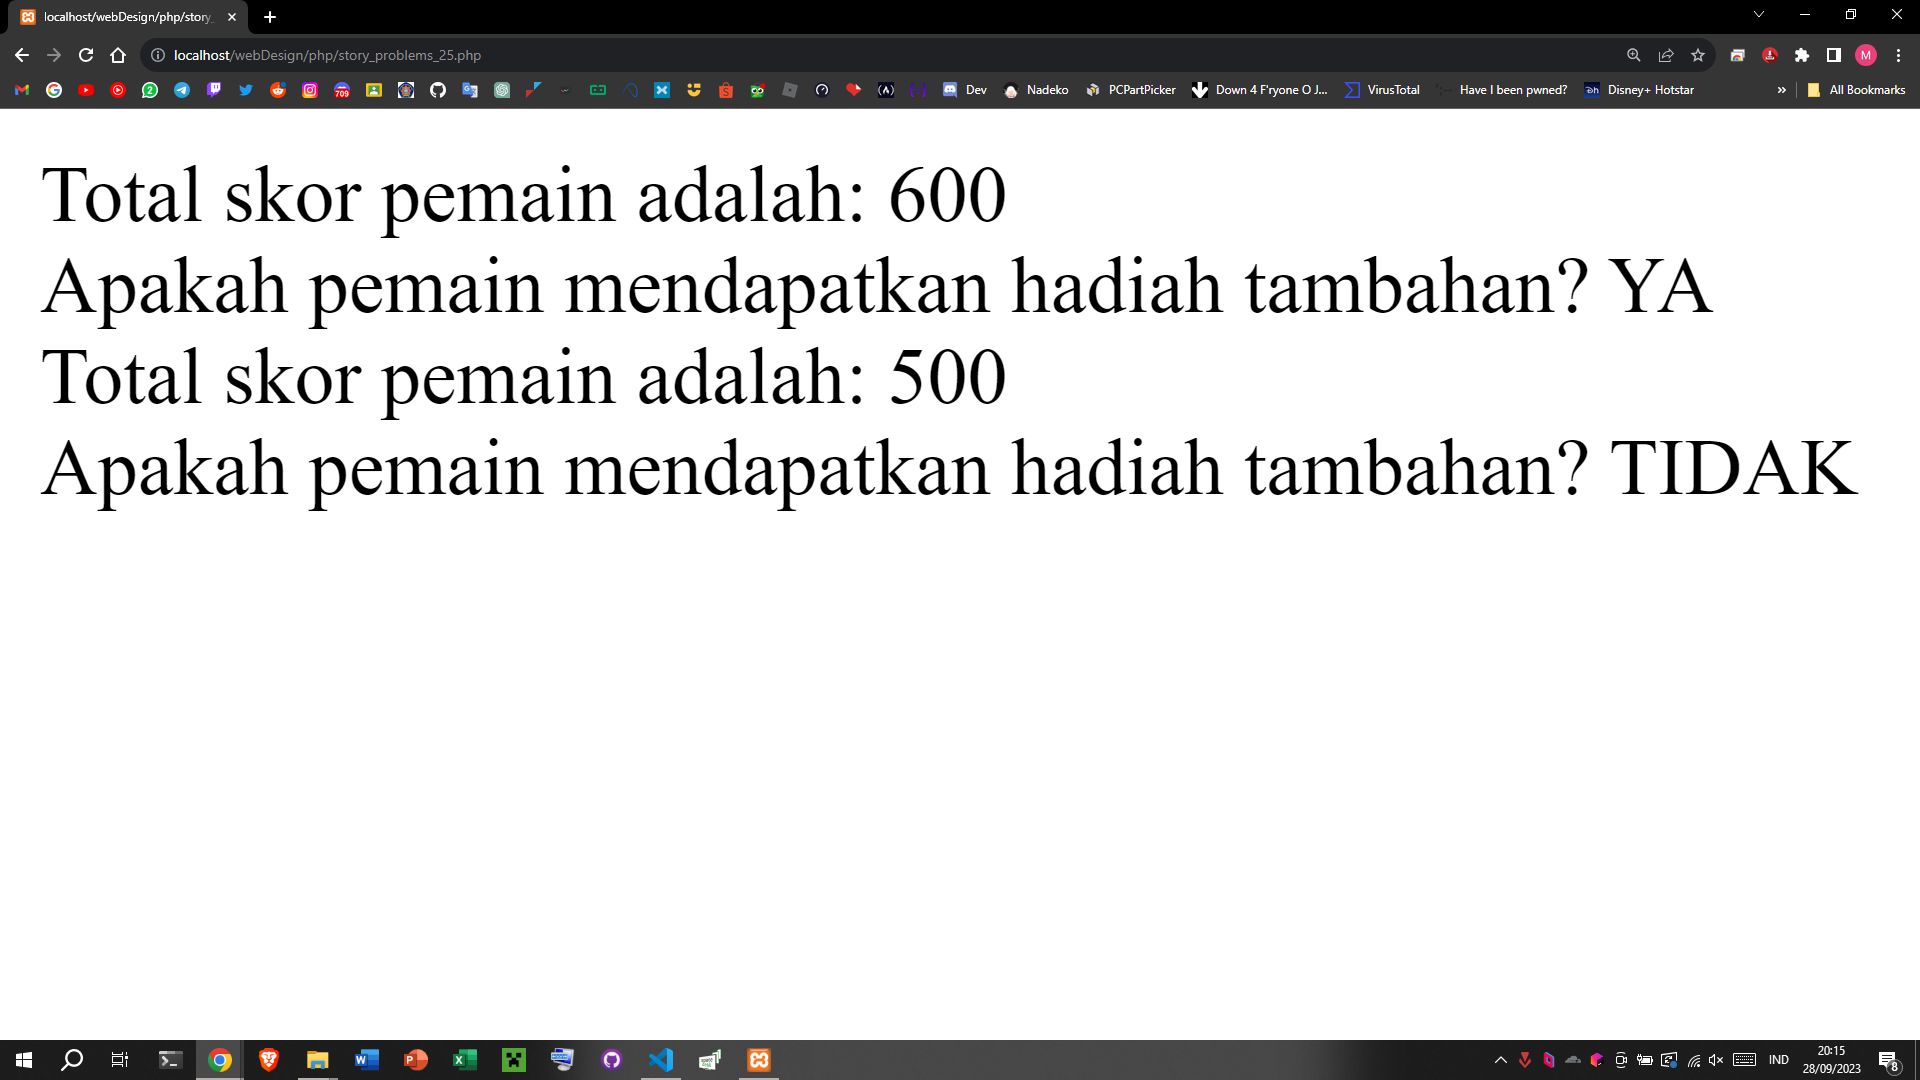
\includegraphics[width=.9\textwidth]{images/figures/fig15.png} \\ one can compare variables with comparison operator and get true or false value from it.
    \newpage
    \item - \\ \includegraphics[width=.9\textwidth]{images/figures/fig16.png} \\ one can store data in an array and then called it with its index in the array to get the data.
    \subsection*{Practicum 8 - Operators}
    \item - \\ 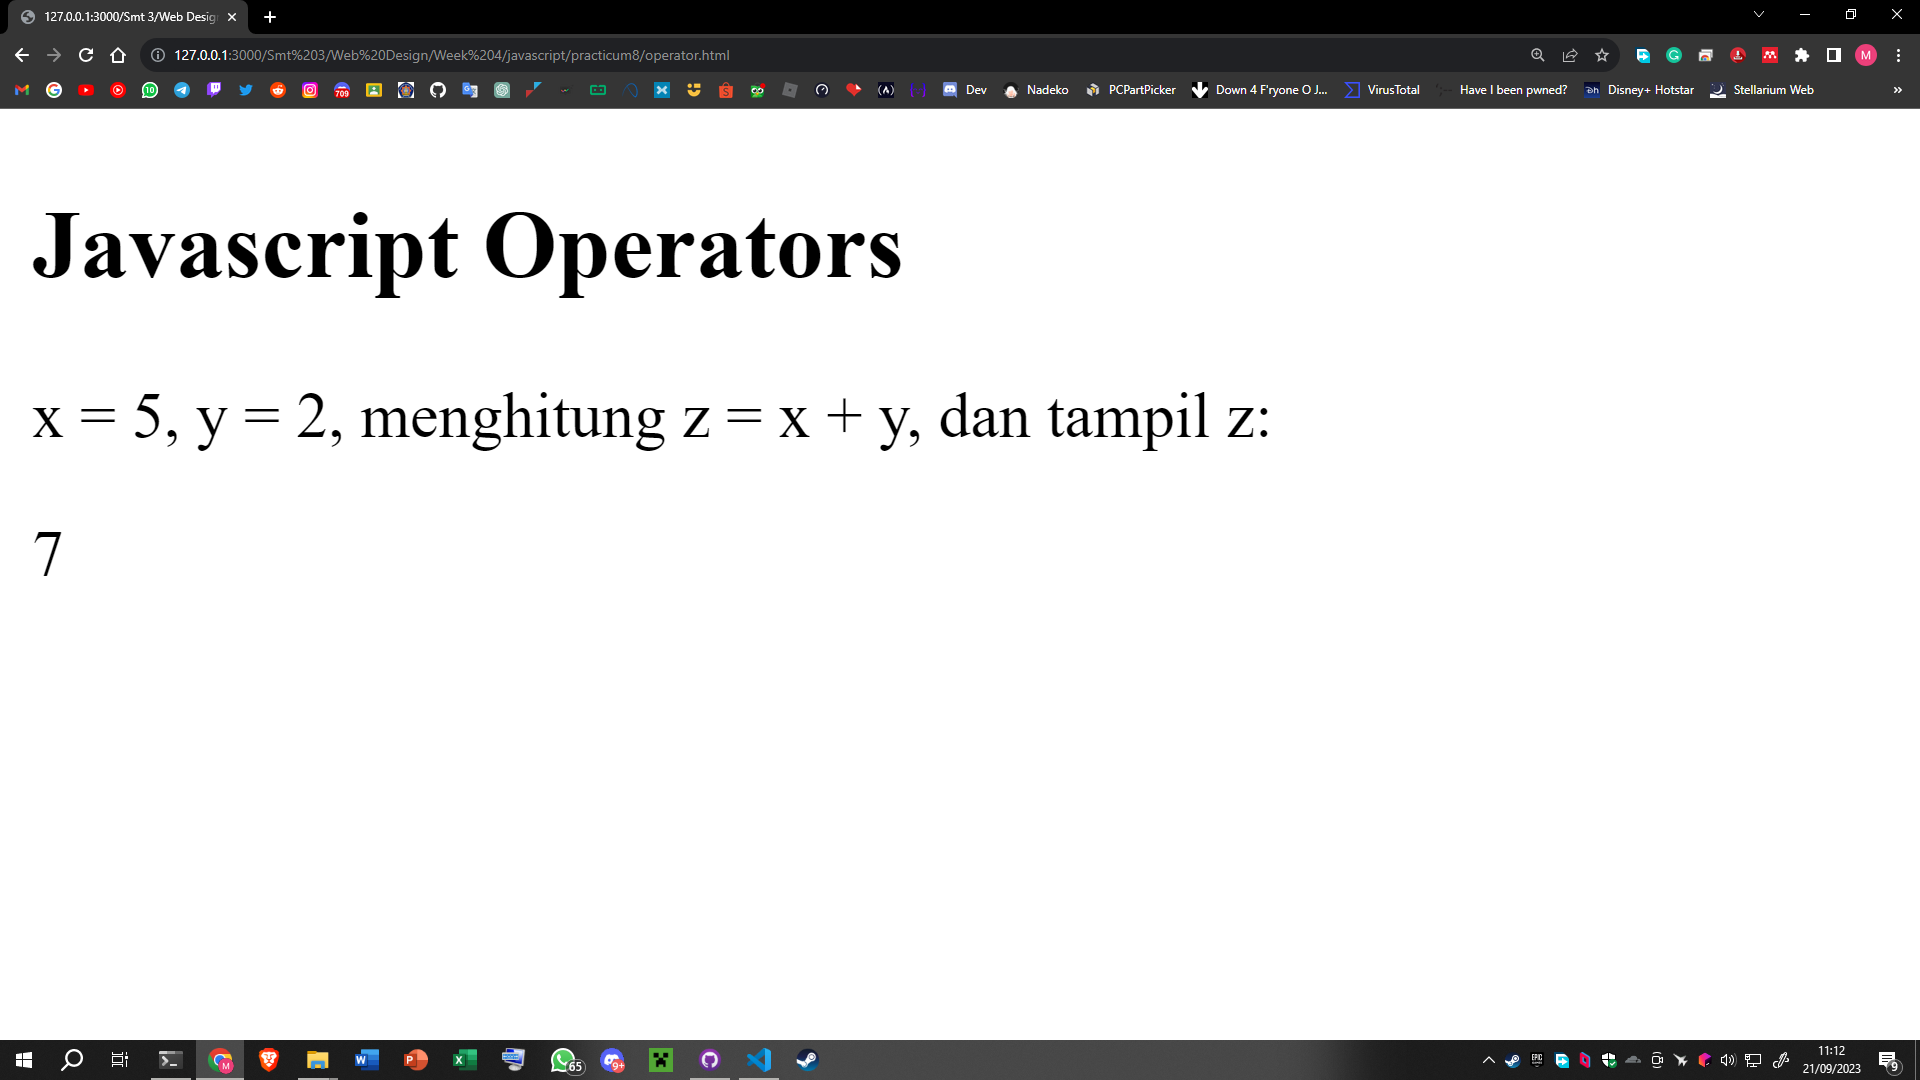
\includegraphics[width=.9\textwidth]{images/figures/fig17.png} \\ the javascript can do operation on the fly.
    \subsection*{Practicum 9 - Selections}
    \subsubsection*{1. Basic If Selection}
    \item - \\ \includegraphics[width=.9\textwidth]{images/figures/fig18.png} \\ when the condition of the if is fulfilled, the code block inside of it run.
    \subsubsection*{2. If Else Selection}
    \item - \\ 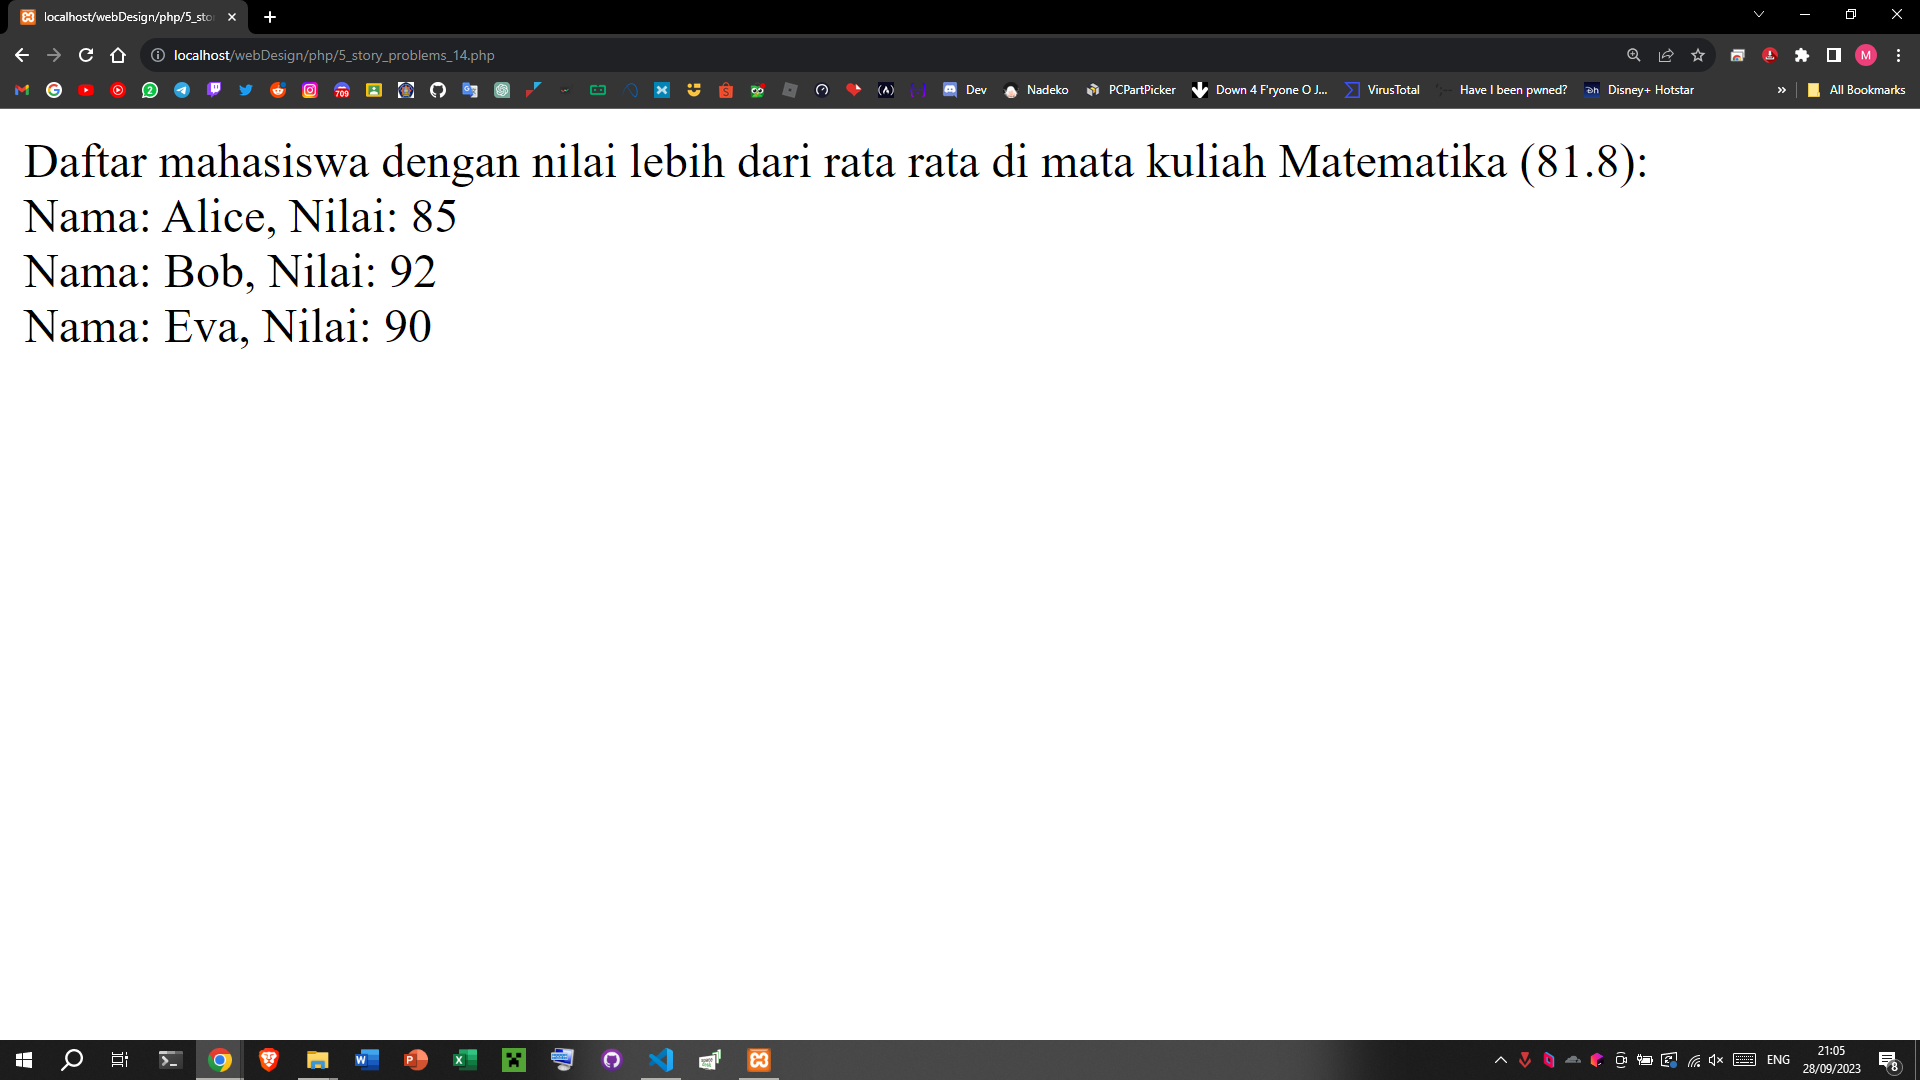
\includegraphics[width=.9\textwidth]{images/figures/fig19.png} \\ now if the condition isn't met the else code block run.
    \subsubsection*{3. Switch Case Selection}
    \item - \\ 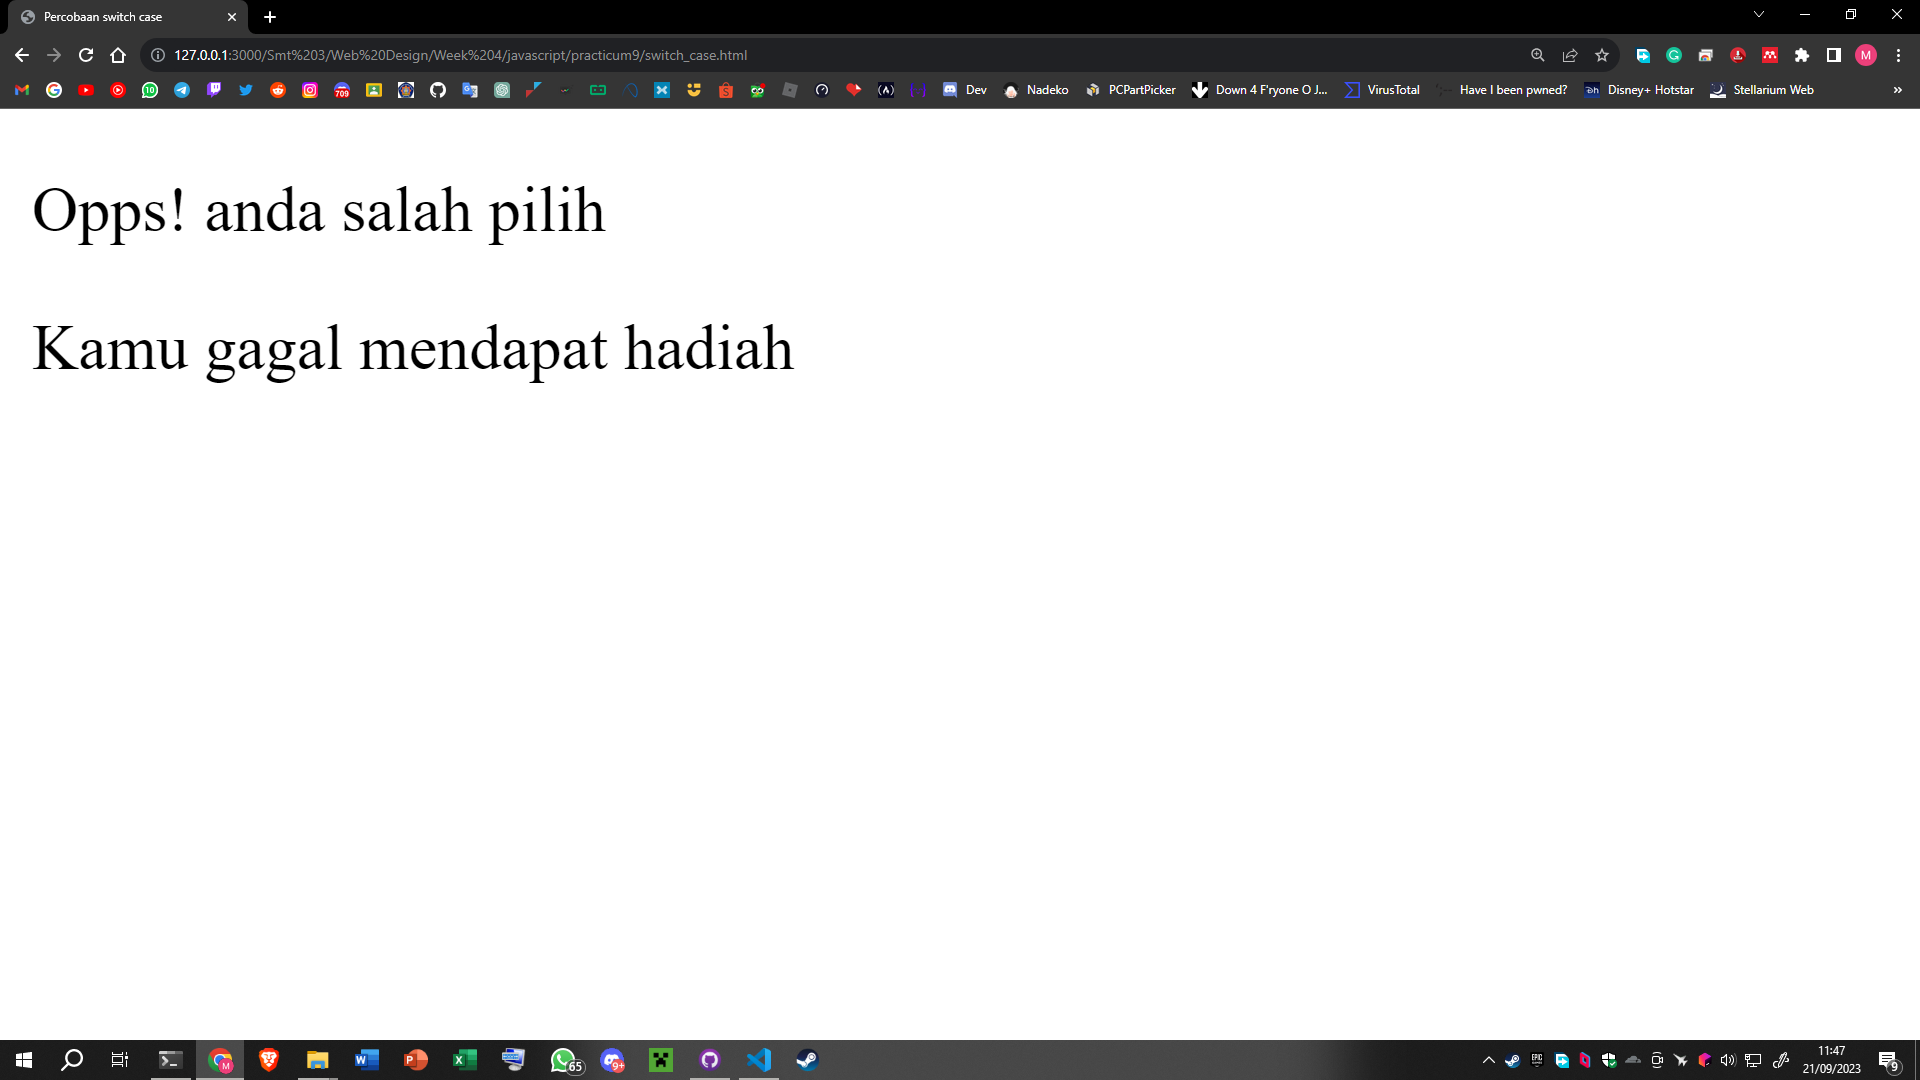
\includegraphics[width=.9\textwidth]{images/figures/fig20.png} \\ the switch case has the ability to run a code block multiple specific condition and run default code block when no case condition isnt met. 
    \subsubsection*{4. Nested Selection}
    \item - \\ 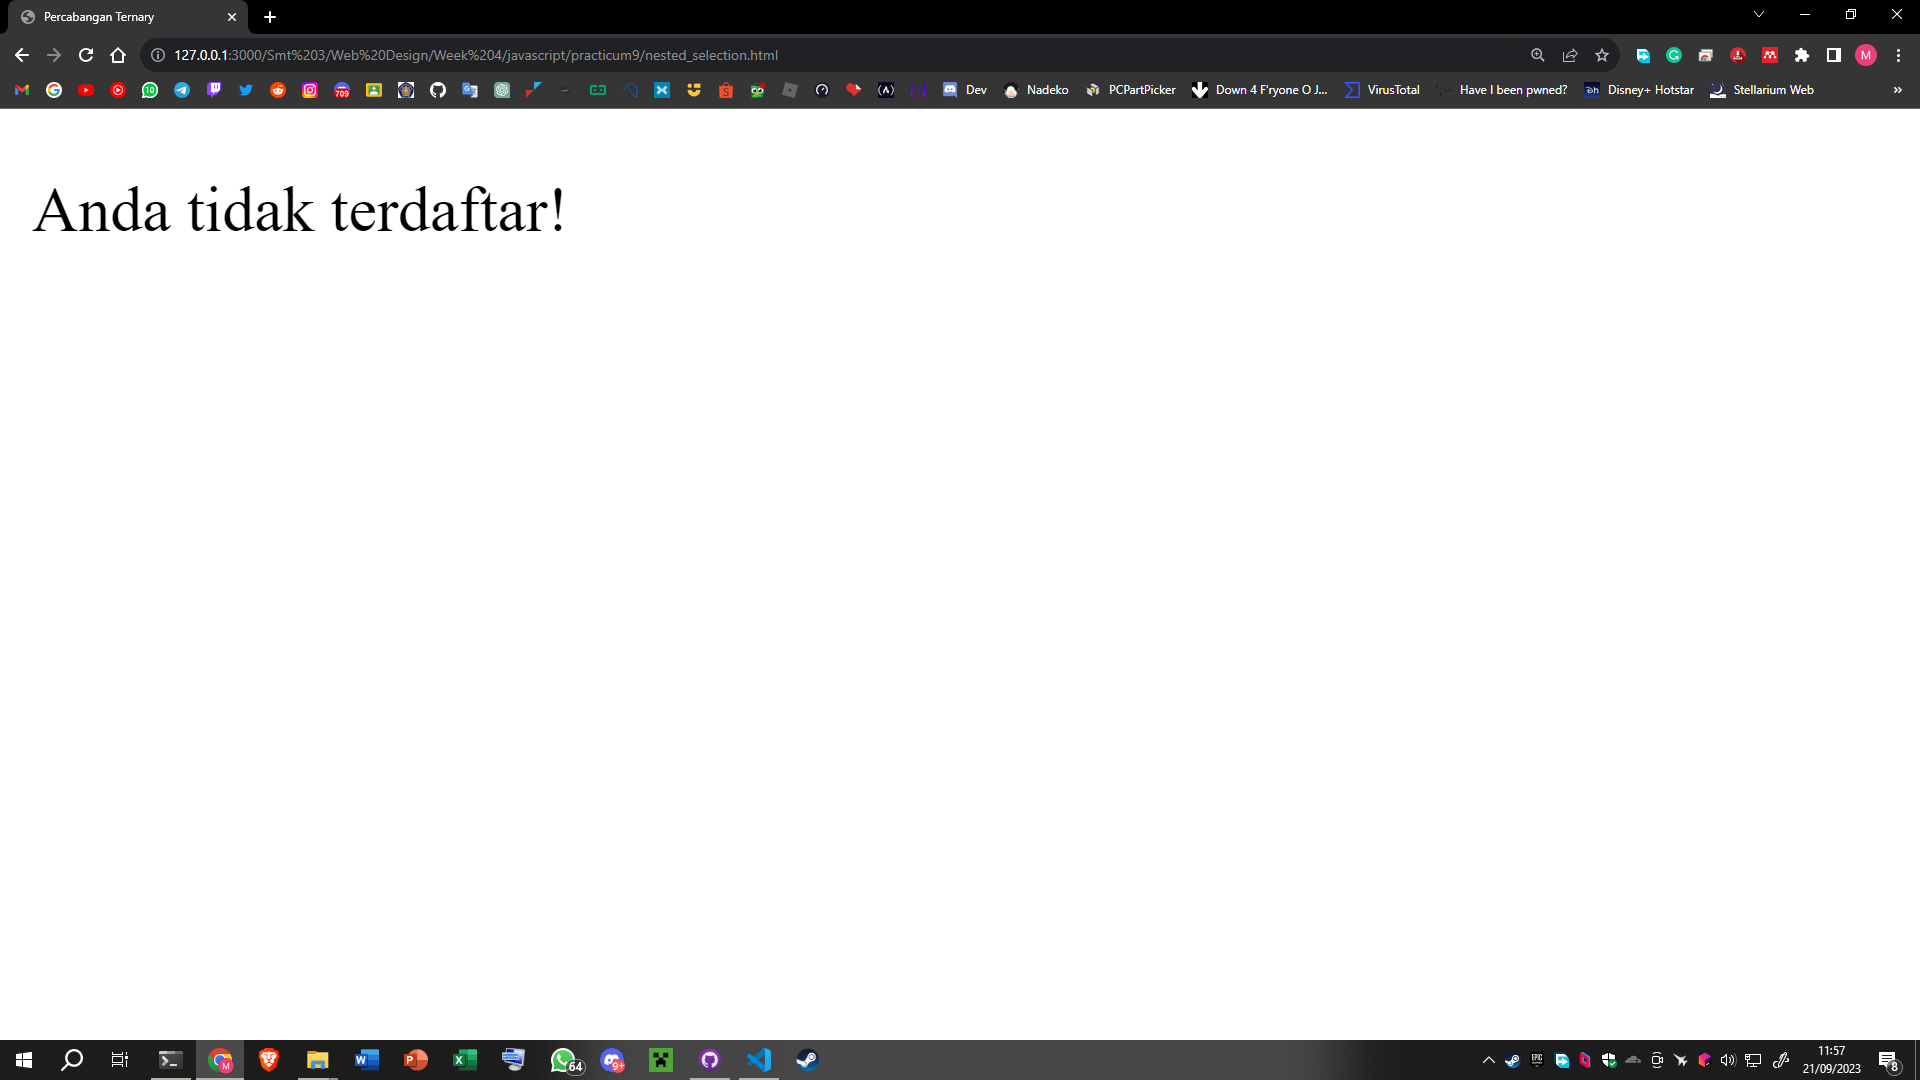
\includegraphics[width=.9\textwidth]{images/figures/fig21.png} \\ the Program check multiple times because there is if inside of if.
    \subsection*{Practicum 10 - Looping}
    \subsubsection*{1. For Loop}
    \item - \\ \includegraphics[width=.9\textwidth]{images/figures/fig22.png} \\ the number got printed 5 times as the looping dictated.
    \subsubsection*{2. While Loop}
    \item - \\ 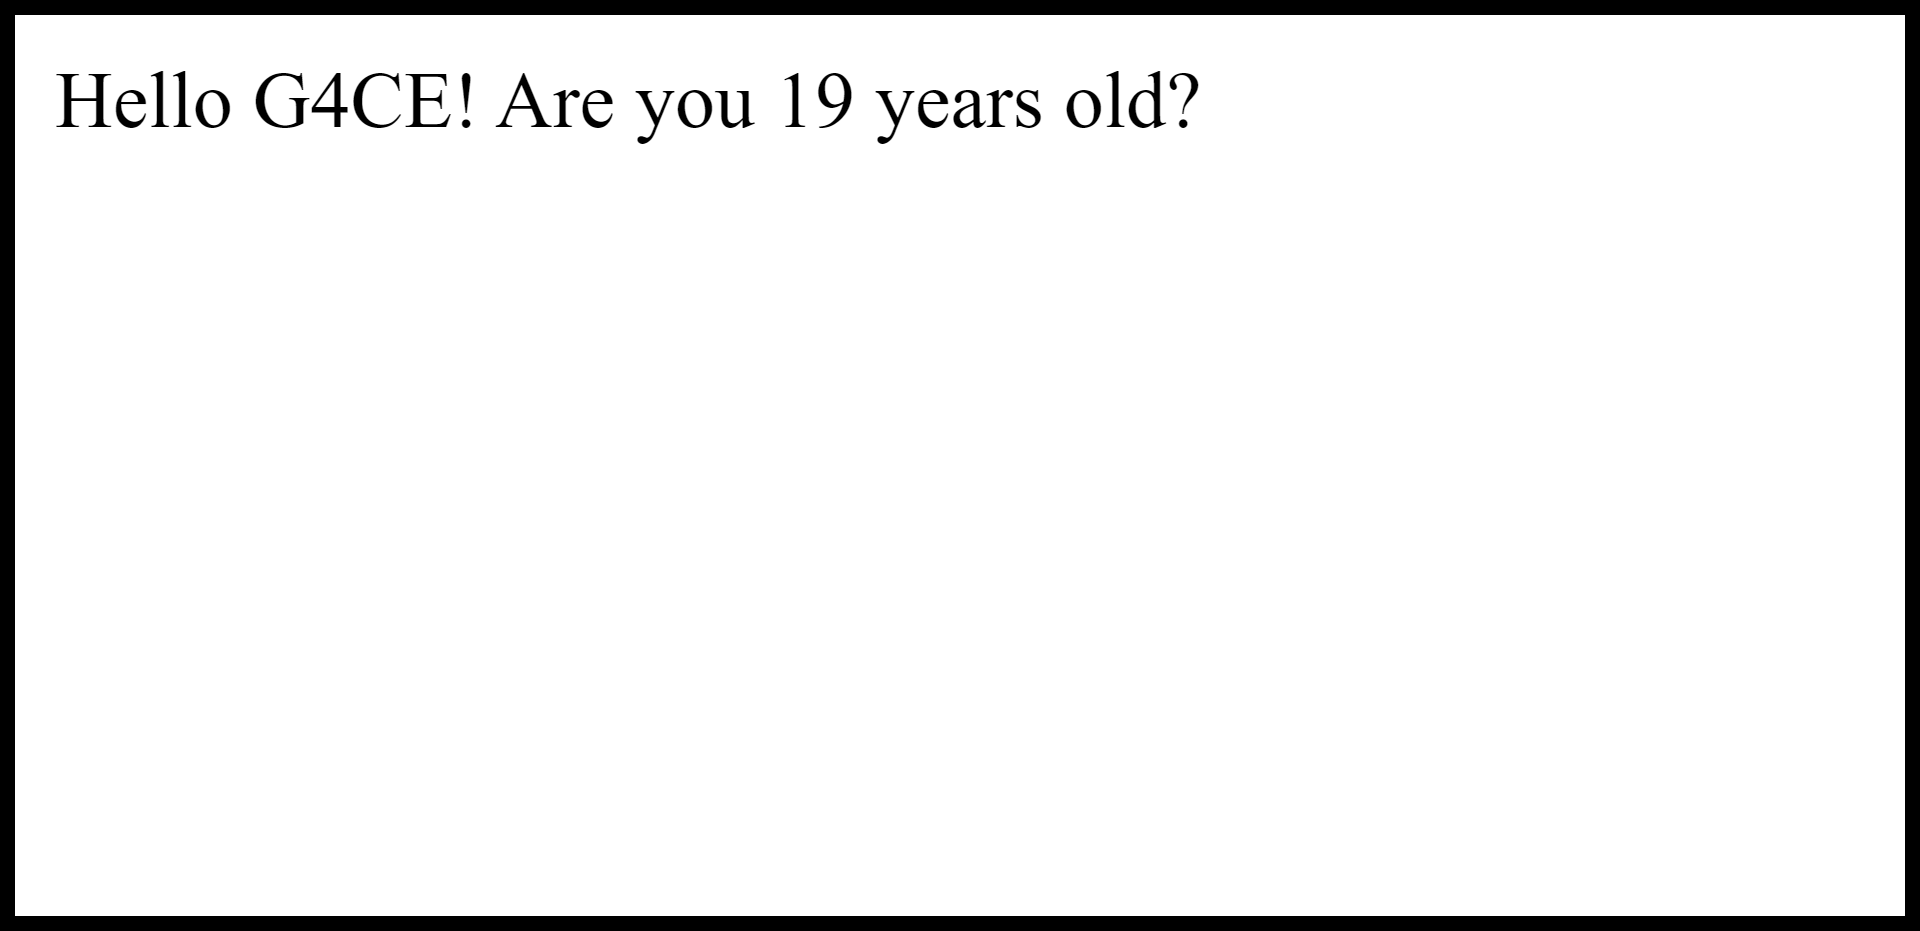
\includegraphics[width=.9\textwidth]{images/figures/fig23.png} \\ it works just like before, but instead of putting variable declaration and increment as 3 statement parameter, we just put the condition then declare and increment manually.  
    \subsubsection*{3. Do While Loop}
    \item - \\ 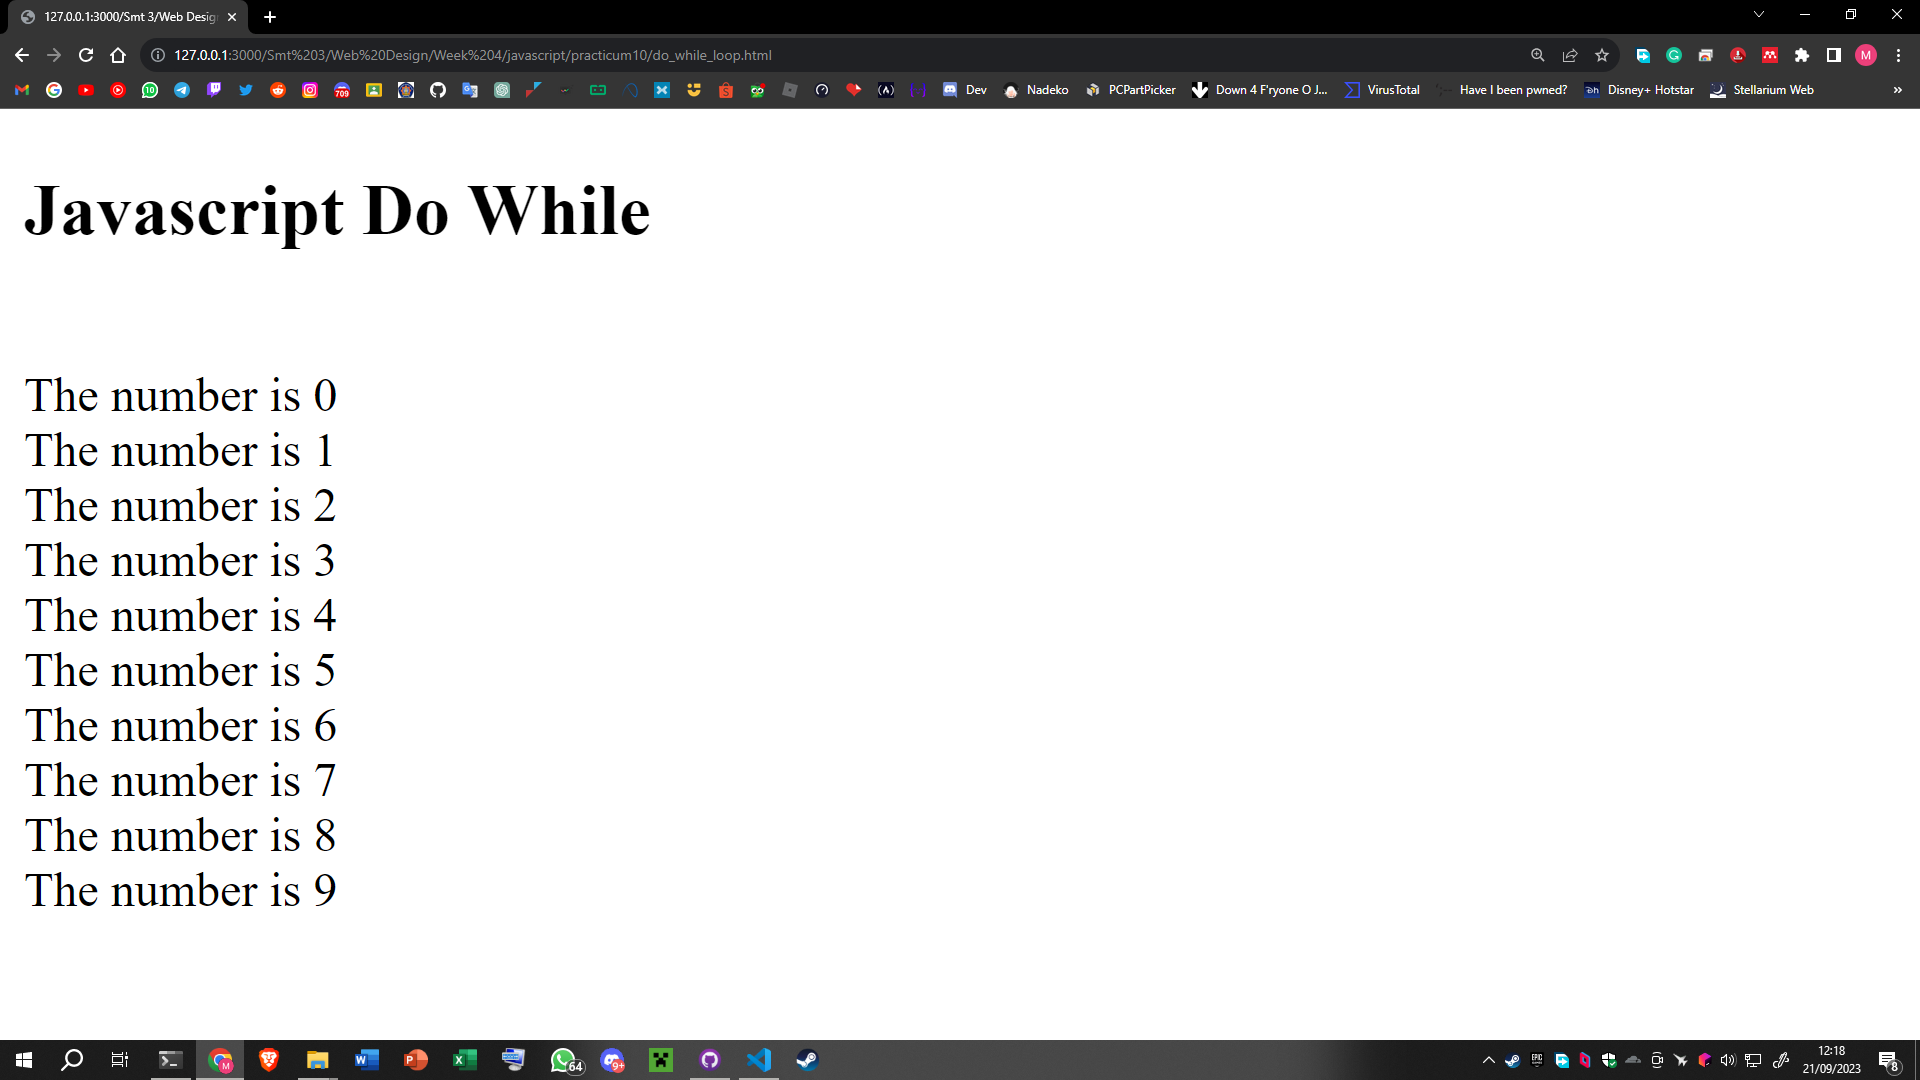
\includegraphics[width=.9\textwidth]{images/figures/fig24.png} \\ it works similarly with while. only different is the do code block is atleast run once before checking the while condition.
\end{enumerate}

\end{document}